In this section, the results in \cite{ArcherSed1} are replicated. Then optimal control problems of the form \eqref{eq:OCP1} are solved.



\subsubsection{Replicating examples from the paper in a periodic box}
The domain in \cite{ArcherSed1} is a box with lengths $L_y = 43.5 \sigma$, and $L_x = 60 \sigma$. 
The strength of the external potential is given by $\beta c = 0.1$ and the strength of the interaction term $\kappa$ is given by $\beta \kappa = - 3.5$, where $\beta = \frac{1}{k_BT}$. 
Furthermore, we have the average density of the system $\bar \rho \sigma^2$, calculated using $(1/L_y)\int_0^L \rho \sigma^2 dy$.
The initial condition for $\rho$ is found by considering $\bar \rho$ and adding a uniform random number to each location in the range $\pm \bar \rho/ 20$. The cases $\sigma \bar \rho = 0.072$ and $\sigma \bar \rho = 0.2$ are considered in \cite{ArcherSed1}.
\\
\\
Since the original simulations are done in a periodic box, we implement the problem in the periodic box as well. We expect near identical results to the paper, given that the setup is identical.
We choose a periodic box that has no flux boundary conditions on the top and bottom of the box, while being periodic on the sides. 
We scale time as done in Equation \eqref{Eq1}, so that the time scales are comparable. In order to get qualitatively good results, we choose $n =100$ and $N = 100$. This takes approximately five hours to solve. In Figure \ref{F5} the results for the configurations corresponding to Figure 8 in Archer's paper can be seen ($ \bar \rho = 0.072$, choosing $\sigma = 1$, and running up to $T = 300$). In Figures \ref{F7} we see the results that correspond to the configurations in Figure 10 in Archer's paper ($ \bar \rho = 0.2$, choosing $\sigma = 1$, running time up to $T = 300$). While the results for Archer's first result look very close to the original, the second set of results is a little different. This may have to do with slightly different initial conditions or numerical solutions.


\begin{figure}[h]
	\centering
	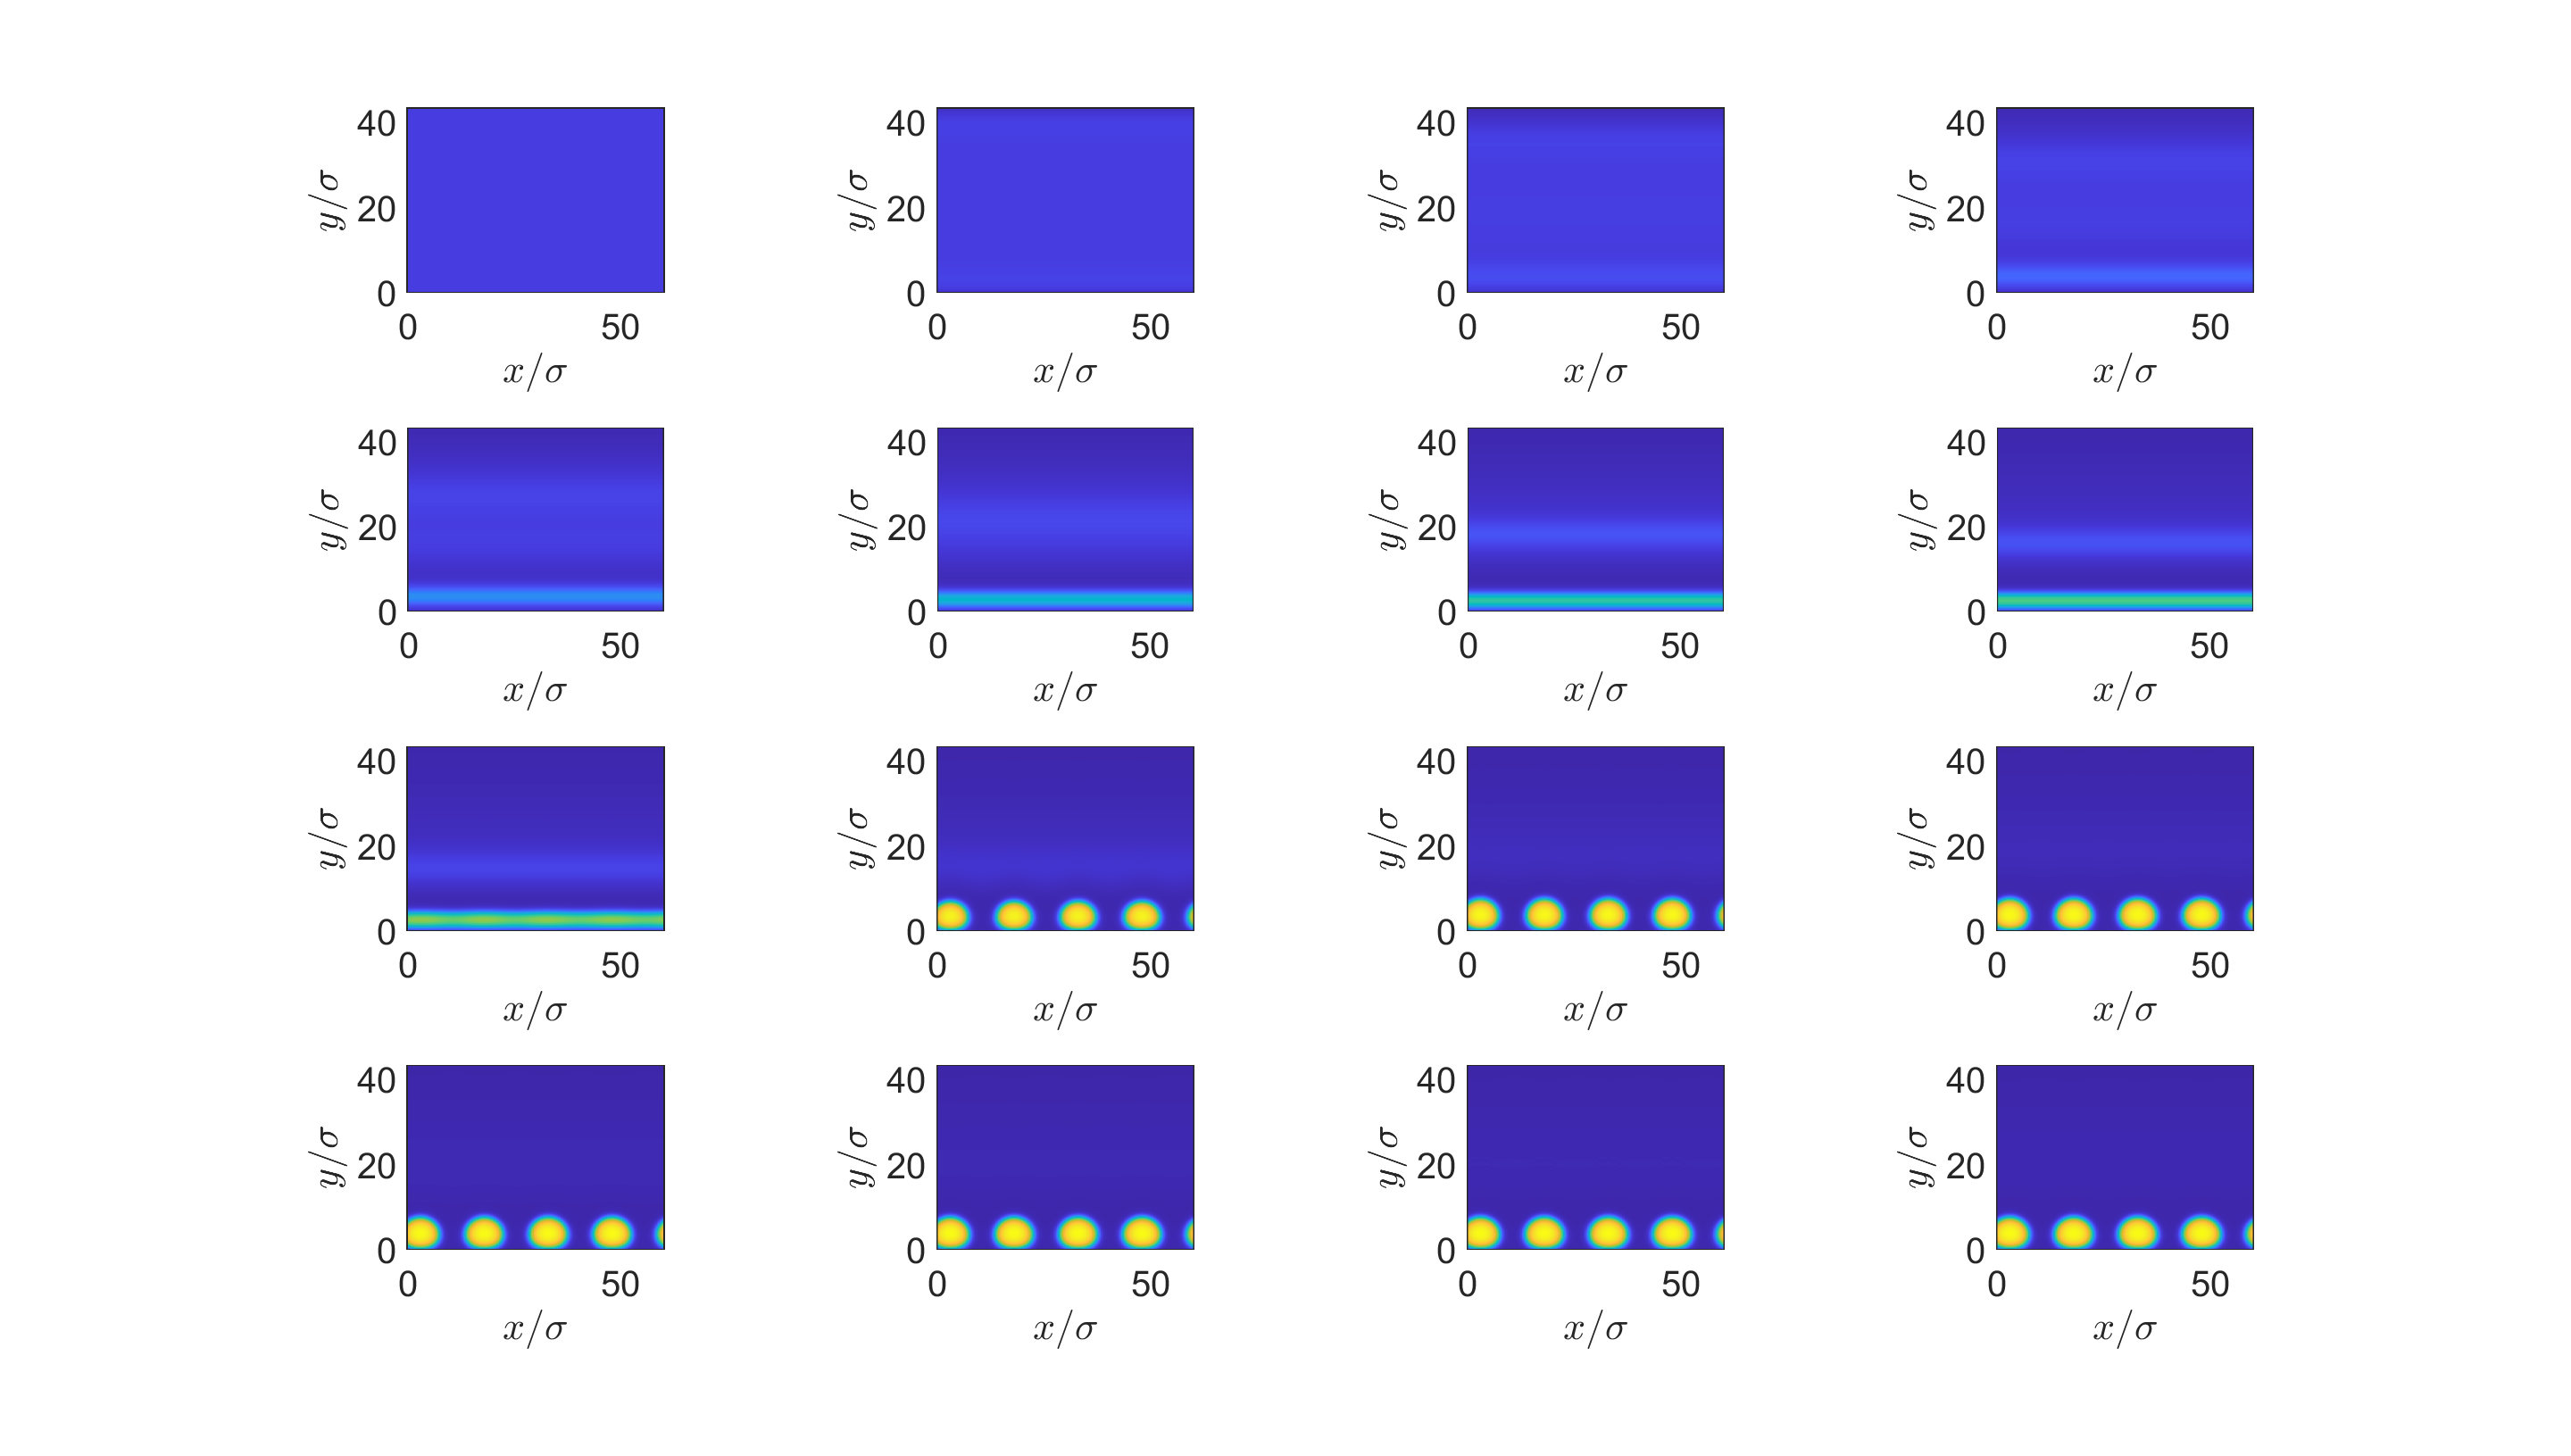
\includegraphics[scale=0.2]{Plotrhobar0072.png}
	\caption{Figure 8 in paper, periodic domain} 
	\label{F5}
\end{figure}
\begin{figure}[h]
	\centering
	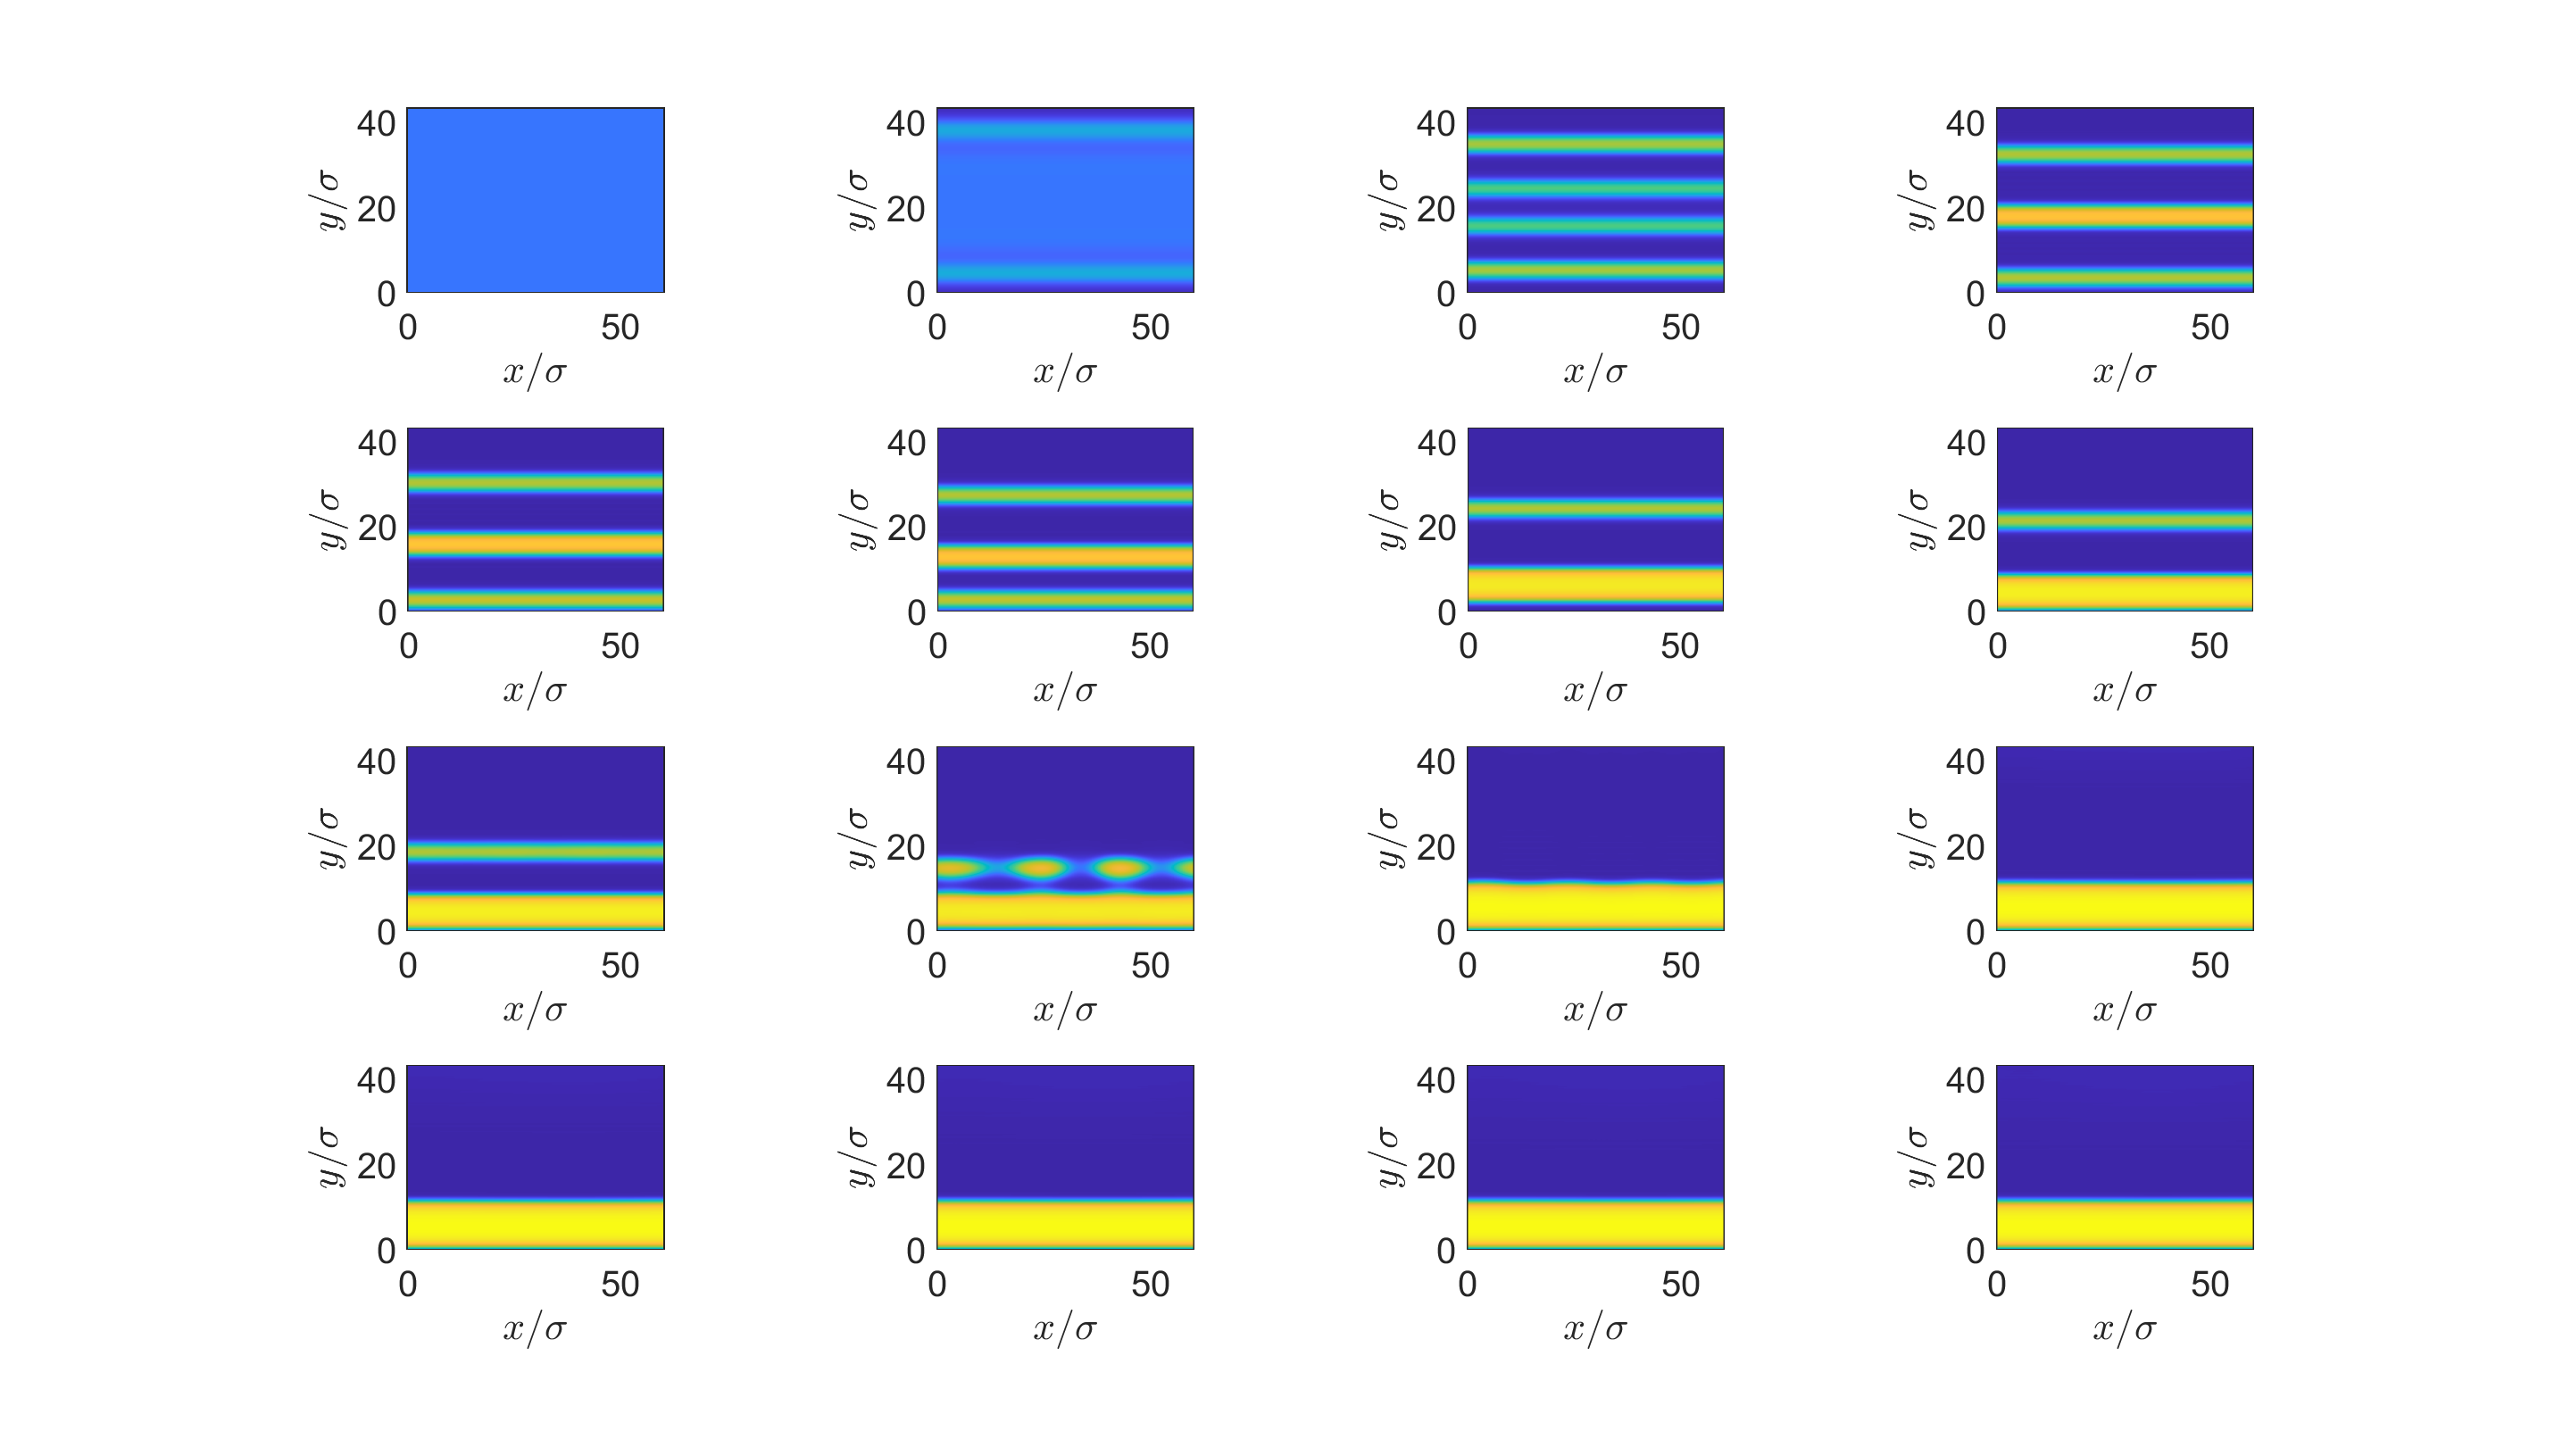
\includegraphics[scale=0.2]{Plotrhobar02.png}
	\caption{Figure 10 in paper, periodic domain} 
	\label{F7}
\end{figure}



\subsubsection{Replicating examples from the paper in a box with noflux BCs}
As above, we choose $N = n = 100$, which takes over 24 hours to run. We run up to time $T = 300$, set $\sigma = 1$ and consider the case $\bar \rho = 0.072$ and $ \bar \rho = 0.2$. Note: the dimensions are switched around, which needs to be fixed with the next rerun. We can see the results for both choices of $\bar \rho$ in Figures \ref{F5b} and \ref{F7b}.

\begin{figure}[h]
	\centering
	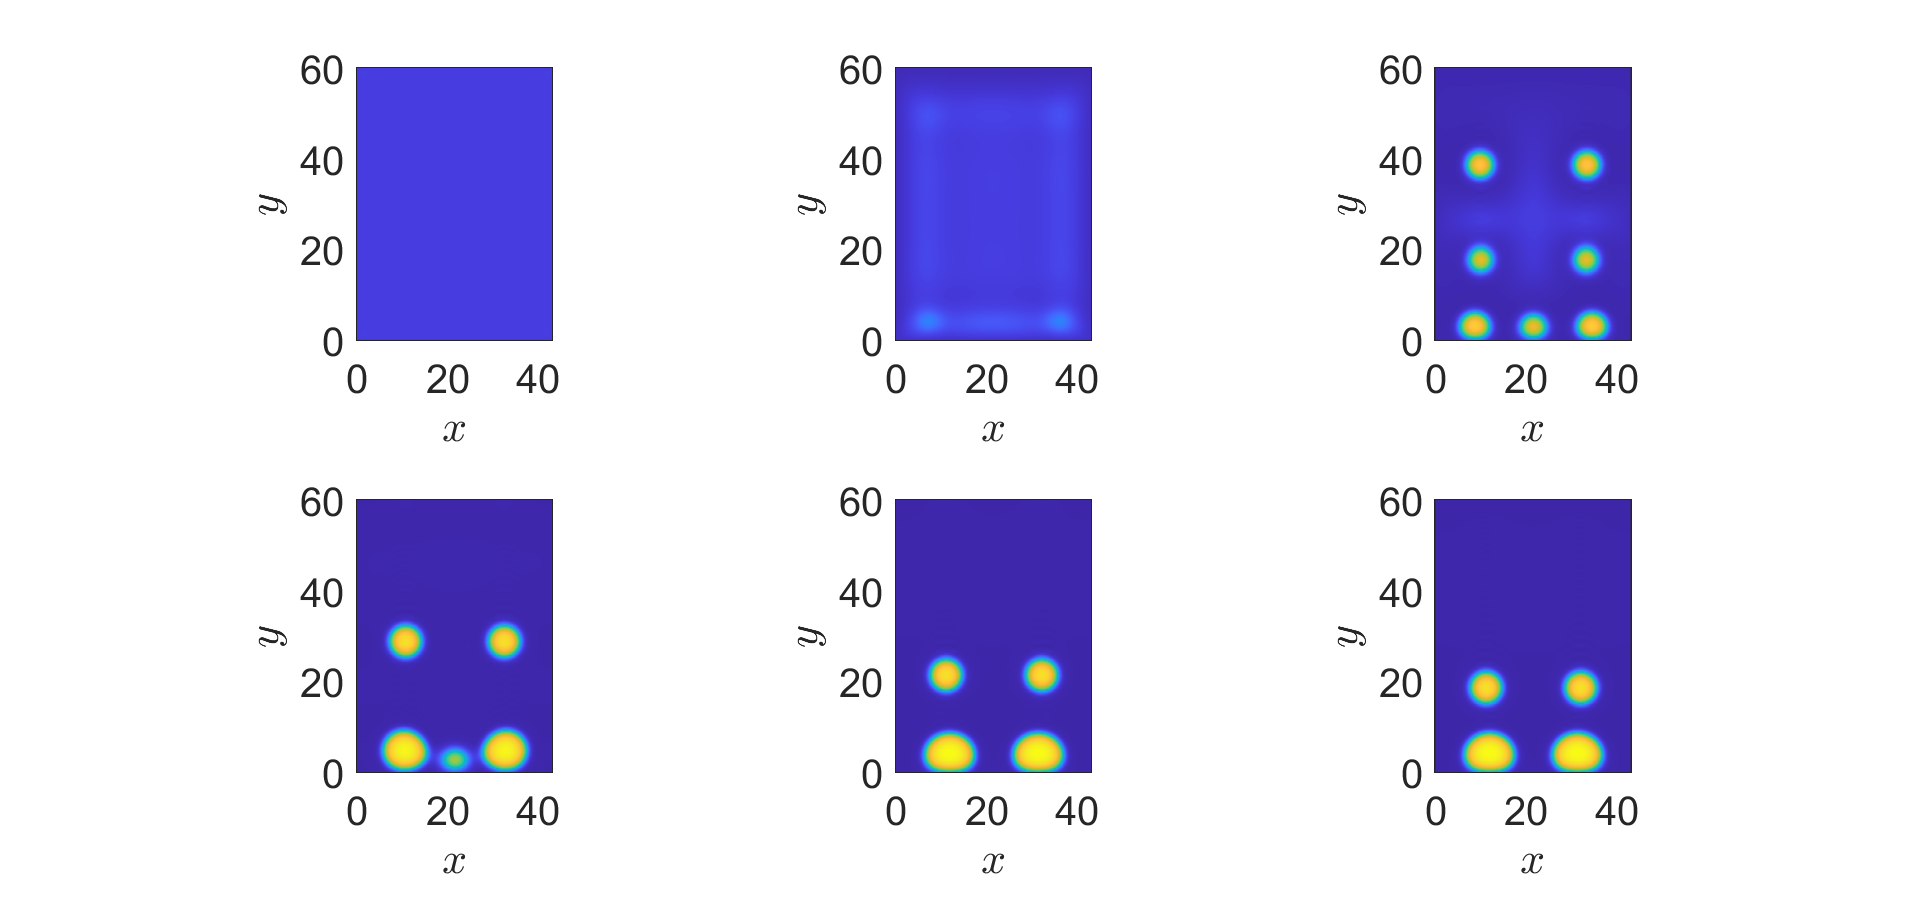
\includegraphics[scale=0.2]{FW0072.png}
	\caption{Figure 8 in paper, no flux BCs, ++ fix wrong dimensions ++} 
	\label{F5b}
\end{figure}
\begin{figure}[h]
	\centering
	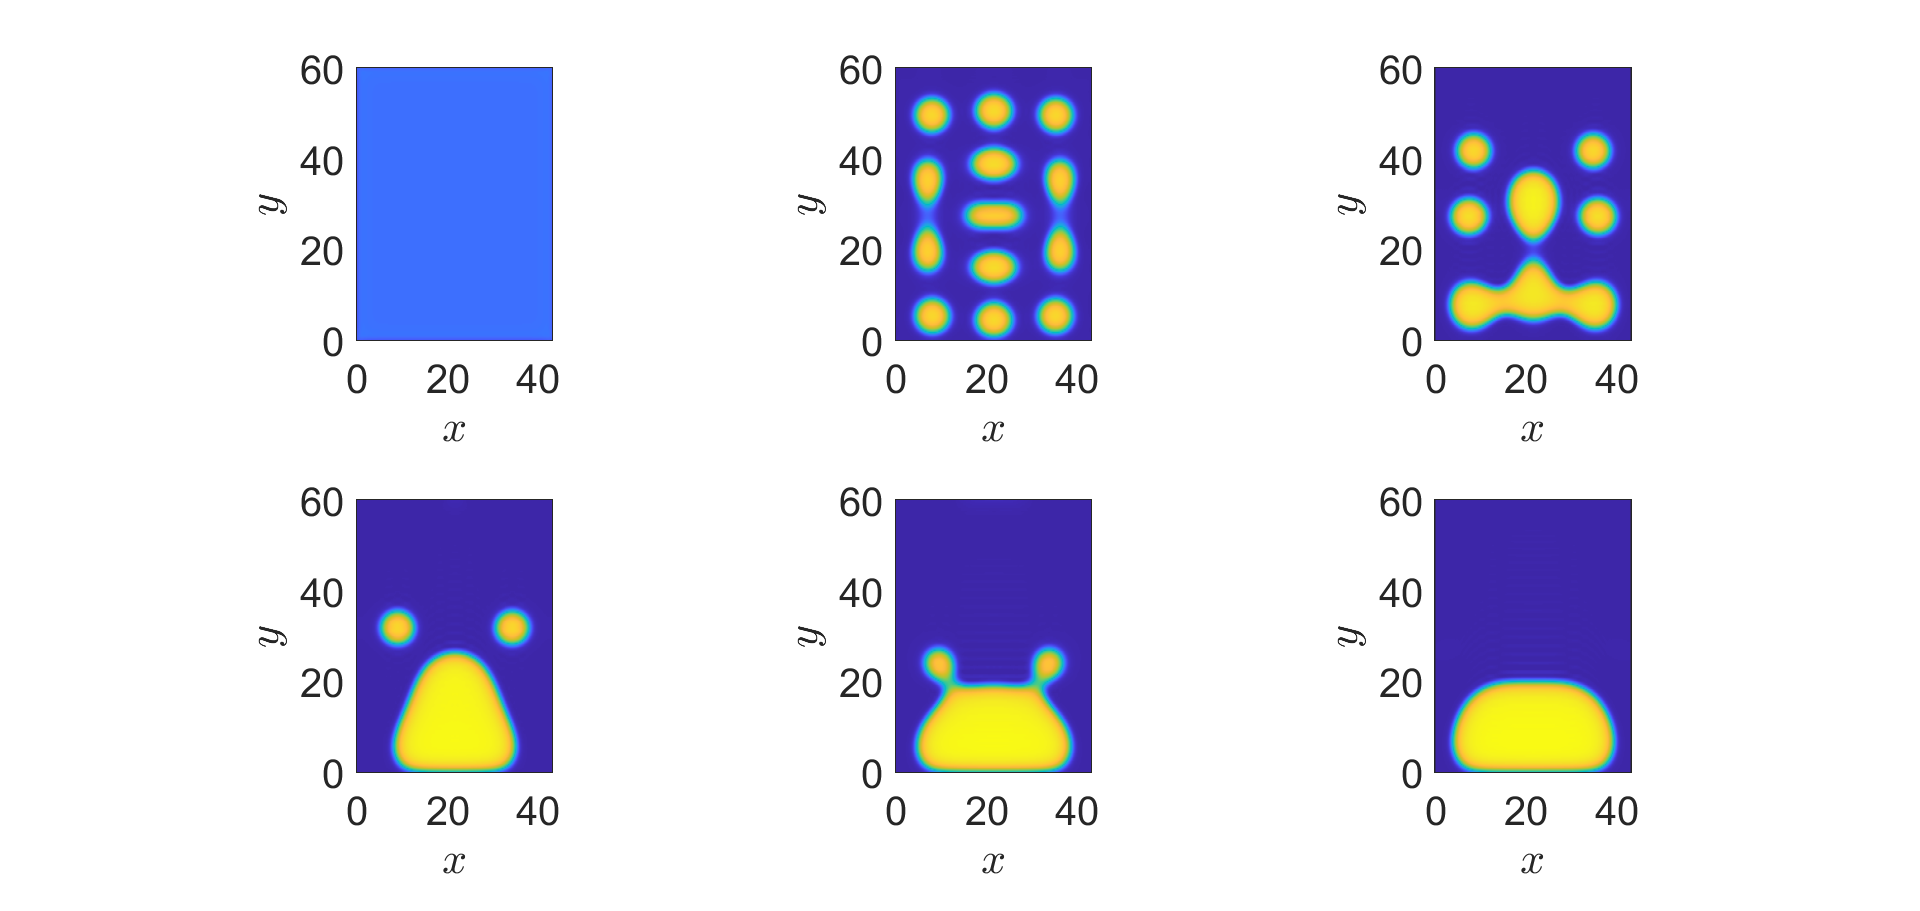
\includegraphics[scale=0.35]{FW02.png}
	\caption{Figure 10 in paper, no flux BCs, ++ fix wrong dimensions ++} 
	\label{F7b}
\end{figure}
